\documentclass[a4wide]{report}

\usepackage{amsmath}
\usepackage[a4paper, total={7in, 10.2in}]{geometry}
\usepackage{graphicx}
\usepackage[portuguese]{babel}
\usepackage[utf8]{inputenc}


\begin{document}

\noindent
{\bf Lincoln Martins de Oliveira (ES 90693)  - Mini-relatório 01 (\today)}

\vspace{0.5cm}

%\section{Introdução}
%\label{intro}

	Os físicos tem um certo desejo por teorias que descrevam os fenômenos da forma mais simples possível. Por esta razão, os modelos de unificação se mostram como alternativas interessantes para a construção de uma física mais simples.
Um dos grandes físicos da história James Clerk Maxwell (Fig.~\ref{pequeno_maxwell}) contribuiu para a unificação entre fenômenos associados a eletricidade e fenômenos associados ao magnetismo.




\begin{figure}[h]
\centering
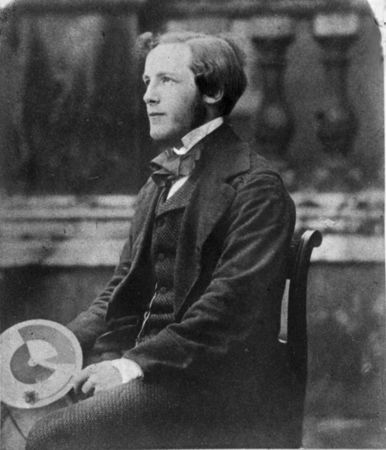
\includegraphics[width=0.23\textwidth]{figure_2}
\caption{A figura mostra uma imagem de Maxwell jovem ~\cite{maxjovem}.}
\label{pequeno_maxwell}
\end{figure}


%\section{Experimentos}
%\label{exp}

	A eletricidade e o magnetismo antes de Maxwell eram descritas pelas seguintes equações.
\begin{equation}
{\bf \nabla} \bullet {\bf E} = \frac{\ro}{\epsilon}
~~~~~~~.
\label{dali_zero_infinito}
\end{equation}
%\begin{eqnarray}
%\nabla \bullet \overrightarrou{E} &=& \left( 1 + \frac{v}{2} \cos \frac{u}{2} 
%\right) \cos u \label{mobius_strip_a} \\
%\nabla &=& \left( 1 + \frac{v}{2} \cos \frac{u}{2} \right) \sin u \label{mobius_strip_b} \\
%\nabla &=& \frac{v}{2} \sin \frac{u}{2} \label{mobius_strip_c}
%\nabla &=& \frac{v}{2} \sin \frac{u}{2} \label{mobius_strip_c}
%\end{eqnarray}
	Por exemplo, tradicionalmente, o bigode do Salvador Dali é descrito pela
seguinte aproximação:
\begin{equation}
\beta \approx \lim_{x\to 0} \frac{1}{x}
~~~~~~~.
\label{dali_zero_infinito}
\end{equation}
	Contudo, além da Eq.~\ref{dali_zero_infinito}, existem teorias alternativas 
que sugerem que o bigode do Salvador Dali é na verdade uma {\bf fita de M\"obius}.
	Uma maneira de representar a fita de M\"obius é utilizando um subconjunto 
no espaço Euclidiano tridimensional definido pela seguinte parametrização~\cite{mobius}:
\begin{eqnarray}
x(u,v) &=& \left( 1 + \frac{v}{2} \cos \frac{u}{2} \right) \cos u \label{mobius_strip_a} \\
y(u,v) &=& \left( 1 + \frac{v}{2} \cos \frac{u}{2} \right) \sin u \label{mobius_strip_b} \\
z(u,v) &=& \frac{v}{2} \sin \frac{u}{2} \label{mobius_strip_c}
\end{eqnarray}
onde $0\leq u < 2\pi$ e $-1\leq v \leq 1$. 
	Outros símbolos matemáticos como os das Eqs. acima são mostrado na Tabela~\ref{simbolos}.

\begin{table}[!h]
\centering
 \begin{tabular}{cccc}
  \hline\\[-0.37cm]
  \hline
 Símbolo    &            Comando                     &  Símbolo  &            Comando                \\ \hline
$\Delta$    & {\ttfamily \textbackslash Delta}       &  $\zeta$  & {\ttfamily \textbackslash zeta}   \\
$\varphi$   & {\ttfamily \textbackslash varphi}      & $\sum_k$  & {\ttfamily \textbackslash sum\_\{k\}}   \\
$\lambda_0$ & {\ttfamily \textbackslash lambda\_\{0\}} &  $\vec{\nu}$    & {\ttfamily \textbackslash vec\{\textbackslash nu\}}     \\
$\hbar$     & {\ttfamily \textbackslash hbar}        &  $\Gamma$ & {\ttfamily \textbackslash Gamma}  \\
$\partial$  & {\ttfamily \textbackslash partial}     & $\int$    & {\ttfamily \textbackslash int}        \\
$\ln$       & {\ttfamily \textbackslash ln}          &  $\#$   & {\ttfamily \textbackslash \#}  \\
$\omega^{-3}$ & {\ttfamily \textbackslash omega\textasciicircum \{-3\}} &  $\nabla$ & {\ttfamily \textbackslash nabla}  \\
$\forall$   & {\ttfamily \textbackslash forall}      &  $\longrightarrow$   & {\ttfamily \textbackslash longrightarrow}  \\
 \hline\\[-0.37cm]
  \hline
\end{tabular}
\caption{Alguns comandos do \LaTeX~comumente utilizados para definir símbolos em expressões matemáticas.}
\label{simbolos}
\end{table}


%\section{Resultados e discussões}
%\label{result_e_discuss}

	Muitas vezes os resultados numéricos que serão obtidos por você durante o curso, 
bem como resultados de experimentos e/ou ilustrações que descrevem o fato/efeito escolhido,
podem ser convenientemente agrupados em uma figura composta.
	Por exemplo, agrupamos na Fig.~\ref{pinturas_de_Dali} as versões ``clássica''
e ``quântica'' dos pinturas de Dali~\cite{dali_paintings}.

~

\begin{figure}[h]
\centering
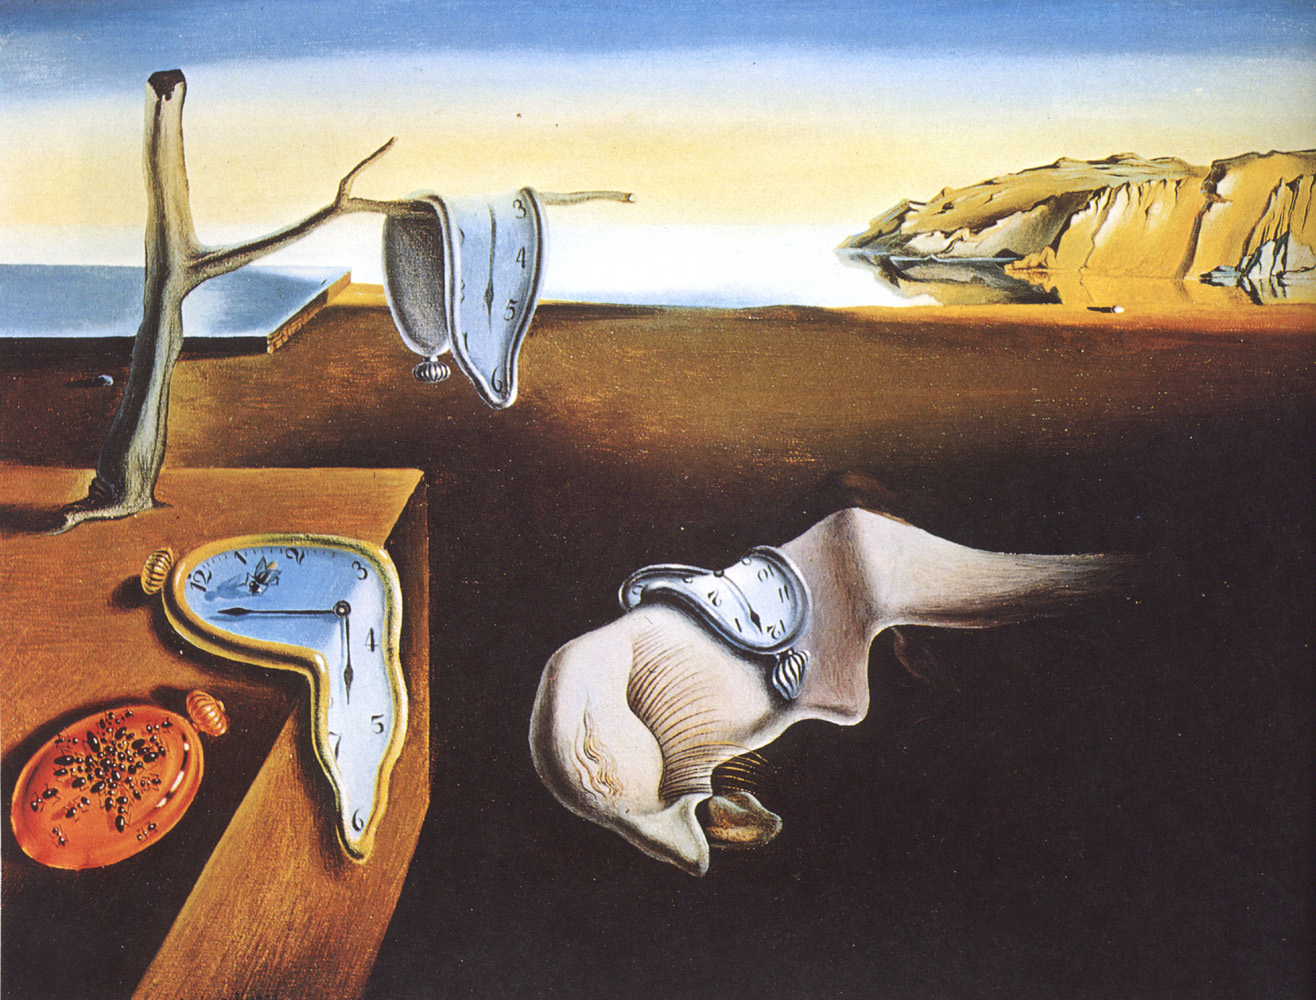
\includegraphics[width=0.45\textwidth]{fig2a_the-persistence-of-memory}%
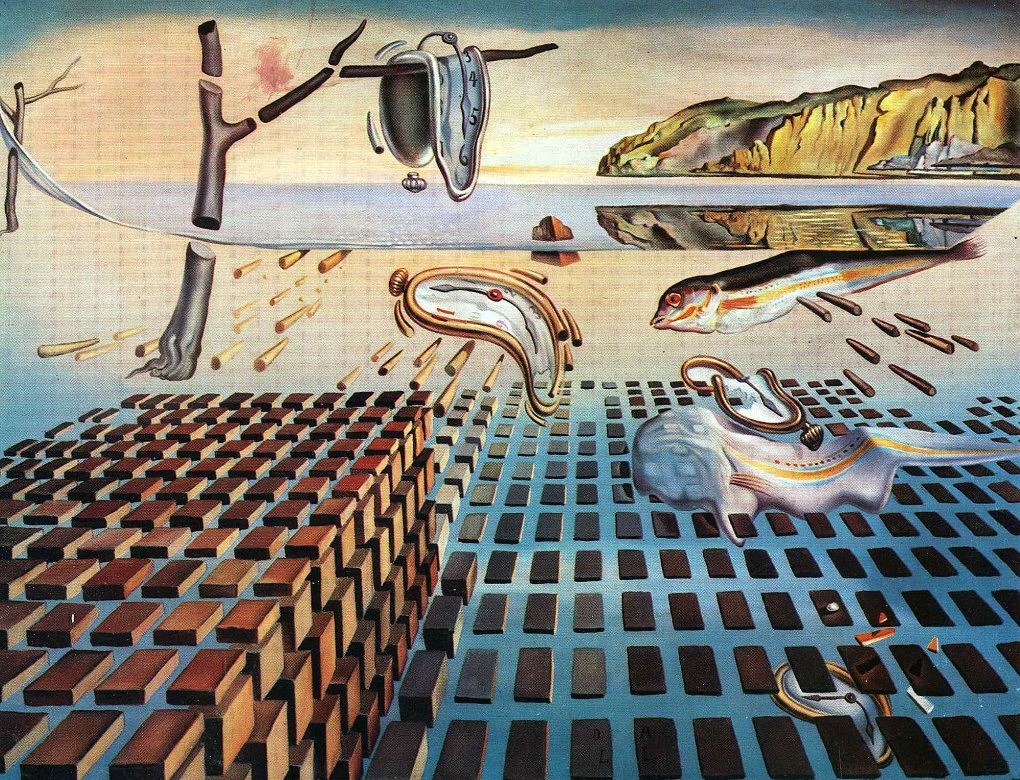
\includegraphics[width=0.447\textwidth]{fig2b_the-disintegration-of-the-persistence-of-memory}
\caption{Pinturas surrealistas de Salvador Dali (veja Ref.~\cite{dali_paintings}): {\it Persistencia de 
la Memoria} (à esquerda) e  {\it La Desintegración de la Persistencia de la Memoria}
(à direita).}
\label{pinturas_de_Dali}
\end{figure}

Finalmente, vale observar que, embora os exemplos contidos nesse documento sejam surreais, 
tenho certeza que o Salvador Dali precisou de muita {\bf lógica}, {\bf reflexão} e 
{\bf dedicação} para concluir suas obras. 
	É exatamente isso que é esperado de você durante o curso, tanto em relação ao 
desenvolvimento de atividades quanto à escrita dos mini-relatórios.
	Além disso, informações corretas e bastante relevantes muitas vezes podem não ser 
encontradas facilmente {\it online} através do Google, então vou citar as 
referências~\cite{hill,lavenda} para lembrar que livros na Biblioteca ainda podem ser 
excelentes referências bibliográficas.





\begin{thebibliography}{99}

\bibitem{maxjovem} Fotografia em https://light2015blog.org/2015/06/12/james-clerk-maxwell-the-man-who-changed-the-world-forever-i/ (acesso em: 14/08/2017)

\bibitem{mobius} http://pt.wikipedia.org/wiki/Fita\_de\_M\"obius (acesso em: 08/08/2017)

\bibitem{dali_paintings} http://www.wikiart.org/en/salvador-dali (acesso em: 08/08/2017)

\bibitem{hill} T. L. Hill. {\it An Introduction to Statistical Thermodynamics} (Dover Books on Physics, 1960).

\bibitem{lavenda} B. H. Lavenda. {\it Statistical Physics: A Probabilistic Approach} (John Wiley \& Sons, 1991)


\end{thebibliography}


\end{document}
